\problemname{High-quality Tree}

The binary search tree is one of the most useful data structures in computer
science. Many \mbox{methods} %prevent hyphen
exist to keep them balanced, such as using tree rotations (like in AVL-trees) or randomness (like in treaps).
One thing that these methods have in common is that they are all somewhat slow and complicated.

But this is all about to change! Rob the computer scientist has invented a new method to keep
rooted binary trees balanced, that is much better than the current state-of-the-art. The main idea
is to repeatedly perform an operation Rob calls a \textit{robbery}. One robbery is to take a leaf
from the tree, and remove it. By applying robberies at the right times, Rob is able to keep a tree balanced
in $\mathcal{O}(1)$ amortized time.

Some people have criticised Rob's revolutionary discovery, saying that removing elements from the tree
makes the algorithm incorrect. Rob does not agree that this is a big problem; if you
plan to store $2 \cdot 10^5$ numbers, you probably do not need all of them.
But Rob accepts the criticism and decides to find a way to minimise the number of robberies.

\begin{figure}[h]
  \centering
  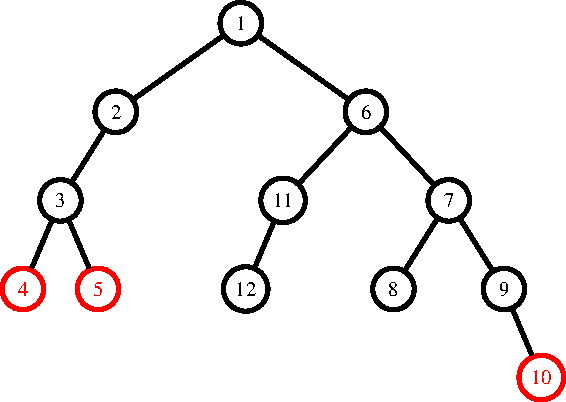
\includegraphics{sample}
  \caption{Illustration of Sample Input 2. The tree becomes strongly balanced
	after removing the three vertices marked in red ($4$, $5$, and $10$);
	the minimum number of vertices that need to be removed to make the tree
	strongly balanced.}
  \label{fig:h}
\end{figure}

You are given a rooted binary tree with $n$ vertices. The vertices are numbered from $1$ to $n$,
and vertex $1$ is the root. Your task is to find the minimum number of robberies to make the tree
\textit{strongly balanced}, meaning that all of its subtrees are balanced. A rooted
binary tree is called balanced if the depth of its left and right subtrees differ by at most one.
Recall that a robbery is simply to take a leaf and remove it, and doing so may
turn its parent vertex into a leaf. See Figure~\ref{fig:h} for an example.

\clearpage
\begin{Input}
  The input consists of:
  \begin{itemize}
    \item One line with an integer $n$ ($1 \leq n \leq 2 \cdot 10^5$), the number of vertices in the tree.
    \item $n-1$ lines, each with two integers $u$ and $v$
          ($1 \leq u, v \leq n$, $u\neq v$), indicating an edge between vertices $u$ and $v$.
  \end{itemize}

  It is guaranteed that the given edges form a valid binary tree with vertex $1$ as the root. However,
  the edges can appear in any order and are not directed: $u$ can be the parent of $v$ or the other way around.
\end{Input}

\begin{Output}
  Output the minimum number of leaves you need to remove to make the tree strongly balanced.
\end{Output}
